	
	
%	\documentclass[11pt,answers]{utfpr-exam}

\documentclass[11pt]{utfpr-exam}	
	

%	\usepackage[hidelinks]{hyperref}
\usepackage{url}
\usepackage{booktabs}
\usepackage{caption}
% Dados

\data{\today} 
\disciplina{ET52B -- Eletrônica Analógica -- Laboratório}
\tipoexame{Roteiro XX: Título do experimento }
\semestre{2018/1}
\professor{Prof. Adriano Ruseler, Dr. Eng.}
\departamento{Departamento Acadêmico de Eletrotécnica -- DAELT}
\universidade{UNIVERSIDADE TECNOLÓGICA FEDERAL DO PARANÁ}	

	
	%==============================================================
\begin{document}

%\imprimircabecalho	
\imprimircabecalholista

\imprimirtabela

%\imprimirtabelacombinada

\begin{framed}
\centering \textbf{\imprimirtipoexame} \par
\noindent\begin{minipage}[t]{.45\textwidth}%
		\noindent \textbf{Objetivos:}
		\begin{enumerate}
			\item Objetivo numero 01 é...
			\item Objetivo numero 02 é...
		\end{enumerate}
	\end{minipage}
	\hfill
	\begin{minipage}[t]{.5\textwidth}%
%		\noindent \textbf{Material utilizado:}
		\begin{center}
			%	\captionof{table}{Lista de material utilizado.}
			\resizebox{\textwidth}{!}{ 
				\begin{tabular}{ccc}
					\toprule
					\textbf{Componente} & \textbf{Descrição} & \textbf{Quantidade} \\ \midrule
					Resistores          & \SI{820}{\ohm}, \SI{5}{\W}             & 4                   \\
					Resistor shunt      & \SI{0.1}{\ohm}, \SI{5}{\W}             & 2                   \\
					Diodos              & 1N4007             & 4                   \\
					Capacitor           & \SI{220}{\micro\farad} x \SI{250}{\V}      & 1                   \\
					Conector Borne      &  KRE 2 Vias    & 2                   \\
					Fusível/Porta Fusível     &  \SI{5}{\A}  & 1                  \\
					Placa padrão        & 10x10              & 1                   \\ \bottomrule
			\end{tabular}
			}	
		\captionof{table}{Lista de material utilizado.}
		\end{center}
	\end{minipage}%	
\end{framed}

\begin{questions}
				
				
\question[25]
\label{Q:revisao}
				
			Monte no simulador PSIM a estrutura apresentada em aula, utilizando o bloco contendo a ponte retificadora trifásica.
			
		\begin{parts}									
			\part[05] Verifique que para $\alpha = 0$ a ponte a tiristor se comporta como caso particular da ponte a diodos.
			\part[10] Obtenha a tensão na resistência de carga.
			\part[10] Calcule os valores eficazes e médios das correntes nos tiristores para $\alpha=60$.	
			\bonuspart[2 \half] What famous mathematician had an elegant proof for this theorem but there was not enough space in the margin to write it down?	
		\end{parts}
							
							
\begin{figure}[!ht]
	\centering
	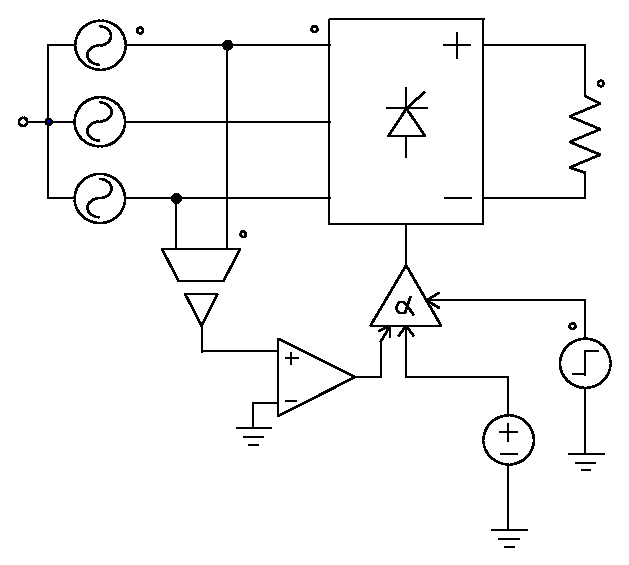
\includegraphics[width=0.5\linewidth]{figuras/SimularEstruturaBloco}
	\caption{Estrutura simulada em Aula.}
	\label{fig:SimularEstruturaBloco}
\end{figure}
			

\begin{solution}
	Once upon a midnight dreary, while I pondered, weak and weary,
	Over many a quaint and curious volume of forgotten lore--- While I
	nodded, nearly napping, suddenly there came a tapping, As of some
	one gently rapping, rapping at my chamber door. ‘‘\,’Tis some
	visitor,’’ I muttered, ‘‘tapping at my chamber door--- Only this
	and nothing more.’’
\end{solution}
			
			
			
			
			
			
	
				
				\question[06]
				\label{Q:perunit}
	Implemente o exercício \ref{Q:revisao} utilizando componentes discretos conforme a figura \ref{fig:TiristorDiscreto}.
	
	\begin{figure}[!h]
	\centering
	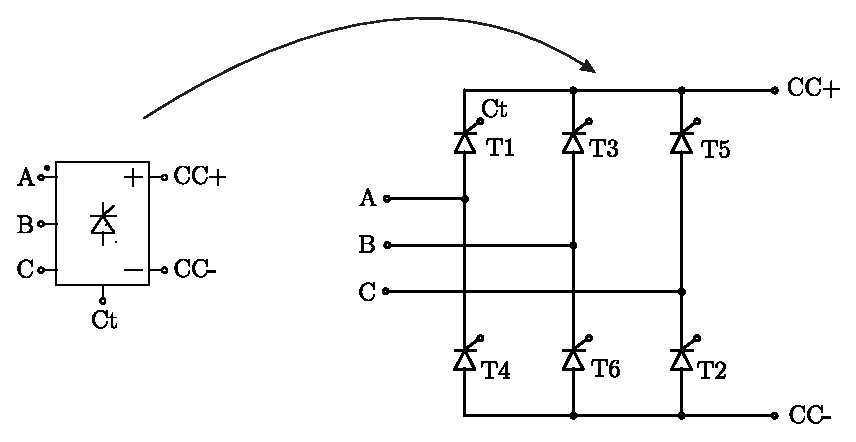
\includegraphics[width=0.7\linewidth]{figuras/TiristorDiscreto}
	\caption{Implemente a versão discreta do retificador trifásico a tiristor.}
	\label{fig:TiristorDiscreto}
	\end{figure}
	

				
							
				\question[07]
				\label{Q:ExPSIM}
				
				
		\begin{figure}[!h]
	\centering
	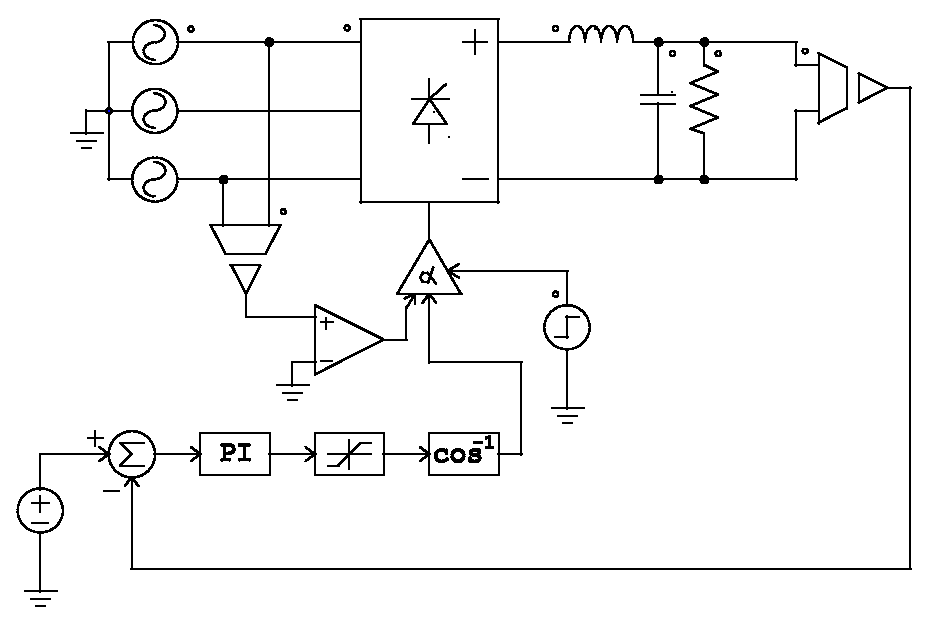
\includegraphics[width=0.7\linewidth]{figuras/ExPSIM}
	\caption{Exemplo do controle de uma ponte retificadora a tiristores.}
	\label{fig:ExPSIM}
	\end{figure}
			
	O software de simulação PSIM possui uma pasta com exemplos em seu diretório de instalação. Procure o exemplo apresentado na figura \ref{fig:ExPSIM}	e faça uma simulação exploratória.		
				

				
				
				
				\question[8]
				\label{Q:Desafio}
		Monte no simulador PSIM a estrutura pentafásica apresentada na figura com carga resistiva.
		\begin{enumerate}
			\item Verifique que para $\alpha = 0$ a ponte a tiristor se comporta como caso particular da ponte a diodos.
			\item Obtenha a tensão na resistência de carga.
			\item Calcule os valores eficazes e médios das correntes nos tiristores para $\alpha=45$.
		\end{enumerate}
		
		\begin{figure}[!h]
			\centering
			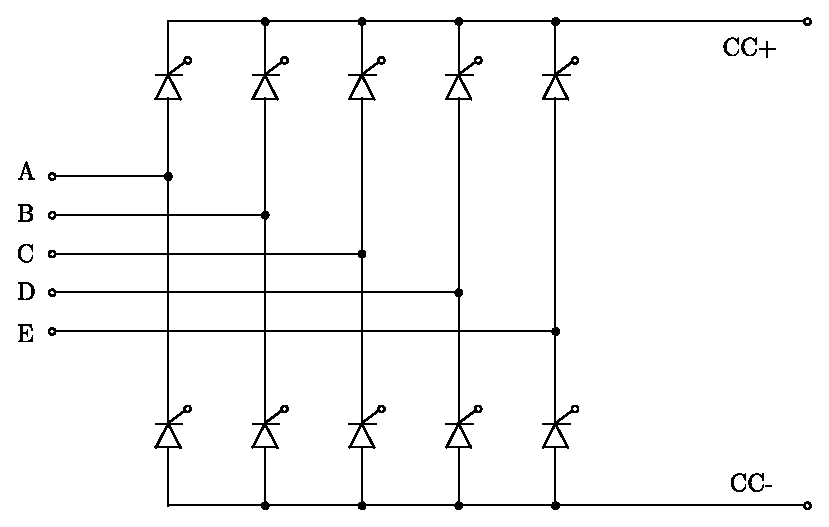
\includegraphics[width=0.7\linewidth]{figuras/TiristorPentafase}
			\caption{Estrutura pentafásica proposta como desafio.}
			\label{fig:TiristorPentafase}
		\end{figure}
				
	
				
	
	\question[20] Considere a expressão $f(x)=3x^3+2x^2+x+1$.
	\noaddpoints % to omit double points count
	\begin{parts}
		\part[10] Calcule $f'(x)$.
		\part[10] Calcule $f''(x)$.
	\end{parts}

	
	\question[2] One of these things is not like the others; one of these
	things is not the same. Which one is different?
	\begin{choices}
		\choice John
		\choice Paul
		\choice George
		\choice Ringo
		\choice Socrates
	\end{choices}
	

	
	\question[3] Mark box if true.
	\addpoints
	\begin{checkboxes}
		\choice 2+2=4
		\choice $\frac{d}{dx} (x^2+1) = 2x+1$
		\choice The Moon is made of cheese.
	\end{checkboxes}
	

	
	\question[10]
	In no more than one paragraph, explain why the earth is round.
	\makeemptybox{\fill}
	
	\newpage
	
	\question[20]
	Explain blah, blah\ldots
	\fillwithlines{\fill}
	
	\newpage
	
	
			
				
		\bonusquestion[30] Prove that the real part of all non-trivial zeros of the function 
		\(\zeta(z)\) is \(\frac{1}{2}\) (A million-dollar question)
			\fillwithdottedlines{8em}
				
				
	
			\end{questions}
%			\begin{center}
%				\rule{.5\textwidth}{1pt}
%			\end{center}
		
		
			
		
		\end{document} 